\documentclass[10pt]{article}
\usepackage{icmlko}

\icmlmeta{IP 파운데이션 월드모델}{225}{나눠 보니 웹툰 하나였다}{판을 두 과제로 갈라 적자마자 챔피언이 갈렸다. 왜 갈리는지 한 칸 더 재니 내가 붙인 이름이 아니었다}

\begin{document}

\twocolumn[
\icmlheader

\begin{abstract}
노트 224가 ``라벨이 두 종류다''를 남기고 남은 것 첫 줄로 ``판을 둘로 적을
것''을 적었다. 적었다(\texttt{lab/rank.by\_kind} --- 순위 규칙은 안
건드리고 나란히 적기만 한다). \textbf{적자마자 판 하나가 덮고 있던 것이
드러난다} --- 판 $\rho$ 로는 F18 배깅 $+$0.4408 이 F21 $+$0.4377 을
간신히 앞서는데, 갈라 보면 \textbf{선호형에서 F18 $+$0.3936 대 F21
$+$0.4236 으로 트리가 지고, 양형에서 $+$0.4715 대 $+$0.4468 로 이긴다.}
0.055 짜리 반전이 하나의 수 뒤에 있었다. 그리고 계열이 통째로 뒤집힌다
--- \textbf{선호형 순위는 선형 셋(F21 · F6 · F9)이 위이고 트리 둘(F18 ·
F8)이 아래인데, 양형은 정확히 반대다.} 다섯 정식화가 두 과제에서 완전히
역순이다. 여기서 멈추면 ``라벨 성질이 모형 계열을 정한다''는 깔끔한
결론이 된다. \textbf{한 칸 더 쟀고 틀렸다.} 도메인별로 F18 $-$ F21 을
보니 \textbf{선호형 두 도메인의 부호가 서로 반대다} --- 웹툰 $-$0.056
인데 \textbf{세계애니는 $+$0.033} 이다. 웹툰이 선호형 유보의 70.3\%
(711/1,011)라 그 하나가 무리 전체를 뒤집는다(가중하면 $-$0.0296 으로
집계와 맞는다). \textbf{선호형 도메인이 둘뿐이라 라벨 성질로 돌릴 수
없다.} 양형 일곱도 부호가 섞인다(도서 $+$0.106 · 펀딩 $+$0.095 · 게임
$-$0.013 · 아이돌 $-$0.180). \textbf{남는 사실은 하나다: 웹툰에서 트리가
선형에 $-$0.056 진다.} 웹툰은 판의 27.7\%로 제일 크고 $\rho$ 가 제일
낮은 도메인이다. \textbf{렌즈는 남기고 이름은 뗀다} --- \texttt{by\_kind}
는 판이 덮는 반전을 드러냈으므로 계속 적되, 그 반전을 ``라벨 종류
때문''이라고 부르지 않는다.
\end{abstract}
]

\begin{figure*}[t]
\centering
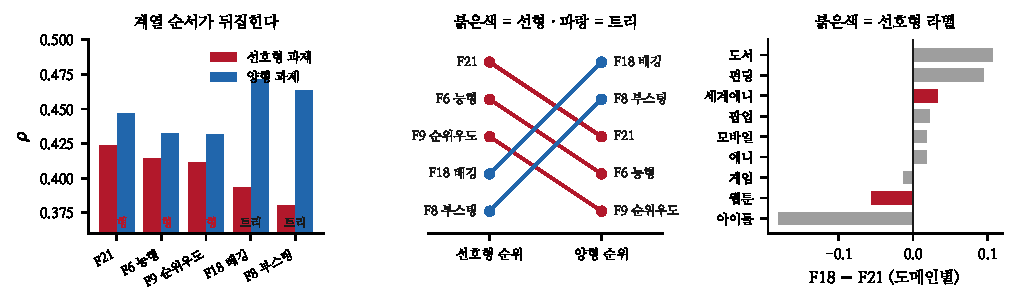
\includegraphics[width=\textwidth]{figs/twoboards.pdf}
\caption{왼쪽 --- 두 과제에서 계열 순서가 뒤집힌다. 가운데 --- 다섯이
완전히 역순이다. 오른쪽 --- 그런데 도메인별로는 선호형 둘의 부호가
반대다.}
\end{figure*}

\section{적자마자 드러났다}

\begin{table}[t]
\centering\tsize
\caption{판을 두 과제로 갈라 적으면(노트 222의 채택 상태).}
\begin{tabular}{lrrrl}
\toprule
& 판 & 선호형 & 양형 & 계열 \\
\midrule
\textbf{F21} & .4377 & \textbf{.4236} & .4468 & 선형 \\
F6 능형 & .4250 & .4140 & .4322 & 선형 \\
F9 순위우도 & .4236 & .4113 & .4316 & 선형 \\
\textbf{F18 배깅} & \textbf{.4408} & .3936 & \textbf{.4715} & 트리 \\
F8 부스팅 & .4305 & .3802 & .4633 & 트리 \\
\bottomrule
\end{tabular}
\end{table}

\claimx{\textbf{판 $\rho$ 하나가 0.055 짜리 반전을 덮고 있었다.} F18 이
판에서 F21 을 $+$0.0031 앞서는데, 선호형에서는 $-$0.0300 지고 양형에서는
$+$0.0247 이긴다.}{\textbf{계열이 통째로 역순이다} --- 선호형은 선형
셋이 위, 양형은 트리 둘이 위. 짝 붓스트랩으로 선호형 최고는 F21, 양형
최고는 F18 이고 \textbf{양쪽 다 나머지 넷이 짝 1 SE 밖}이다.}

\claimx{\textbf{순위 규칙을 안 건드렸다} --- 판정치를 바꾸는 것이 아니라
같은 예측을 둘로 나눠 적는 것이다.}{노트 211이 도메인별 달력 몫을 판 옆에
적자고 하고 안 했다. \textbf{이번에는 값이 안 드는 쪽을 먼저 했고 그
자리에서 나왔다.}}

\section{한 칸 더 재니 틀렸다}

\begin{table}[t]
\centering\tsize
\caption{도메인별 F18 $-$ F21.}
\begin{tabular}{llrr}
\toprule
& 성질 & 유보 & F18$-$F21 \\
\midrule
\textbf{웹툰} & \textbf{선호} & 711 & \textbf{$-$.056} \\
애니 & 양 & 606 & $+$.018 \\
모바일 & 양 & 441 & $+$.019 \\
\textbf{세계애니} & \textbf{선호} & 300 & \textbf{$+$.033} \\
게임 & 양 & 180 & $-$.013 \\
도서 & 양 & 163 & $+$.106 \\
펀딩 & 양 & 80 & $+$.095 \\
팝업 & 양 & 59 & $+$.022 \\
아이돌 & 양 & 25 & $-$.180 \\
\bottomrule
\end{tabular}
\end{table}

\claimx{\textbf{선호형 두 도메인의 부호가 서로 반대다} --- 웹툰 $-$0.056
인데 세계애니는 $+$0.033 이다. \textbf{웹툰이 선호형 유보의 70.3\%}
(711/1,011)라 그 하나가 무리를 뒤집는다(가중 $-$0.0296, 집계
$-$0.0300 과 맞는다).}{\textbf{선호형 도메인이 둘뿐이라 라벨 성질로 못
돌린다.} 양형 일곱도 부호가 섞인다 --- 도서 $+$0.106 · 펀딩 $+$0.095 ·
게임 $-$0.013 · 아이돌 $-$0.180.}

\claimx{\textbf{내가 붙인 이름이 틀렸다.} ``라벨 성질이 모형 계열을
정한다''는 깔끔한 결론이 될 뻔했는데 도메인 하나였다.}{노트 133의
규칙이 또 걸렸다 --- \textbf{첫 양수를 그대로 안 쓴다.} 그리고 이번에는
집계가 아니라 \emph{집계 위에 붙인 해석}이 틀린 경우다. 노트 218이
``결론 옆에 적은 까닭이 결론보다 잘 틀린다''를 여덟 번째로 셌는데
아홉 번째다.}

\claimx{\textbf{렌즈는 남기고 이름은 뗀다.} \texttt{by\_kind} 는 판이
덮는 반전을 드러냈으니 계속 적되, 그 반전을 ``라벨 종류 때문''이라고
부르지 않는다.}{\textbf{남는 사실은 하나다 --- 웹툰에서 트리가 선형에
$-$0.056 진다.} 웹툰은 판의 27.7\%로 제일 크고 $\rho$ 가 제일 낮다
(노트 222의 천장표 1 위).}

\begin{table}[t]
\centering\tsize
\caption{남은 것.}
\begin{tabular}{ll}
\toprule
\textbf{웹툰} & 왜 거기서만 트리가 지나 \\
\textbf{아이돌} & $-$0.180 --- 유보 25건이라 못 믿는다 \\
도메인 표 & 판 옆에 F18$-$F21 도메인별을 상시로 \\
\bottomrule
\end{tabular}
\end{table}

첫 줄이 이 사이클이 세 번째로 웹툰을 가리키는 자리다. 노트 222의 천장표가
웹툰을 1 위로($+$0.1769) 짚었고, 노트 223이 웹툰 축을 찾았다가 노트 224에서
사후로 물렸고, 이 노트는 \textbf{웹툰이 유일하게 트리가 지는 큰
도메인}임을 보인다. \textbf{셋이 같은 곳을 가리킨다} --- 제일 크고, 제일
못 맞히고, 다른 도메인과 다르게 행동한다. 노트 212가 웹툰 라벨(누적
즐겨찾기)을 고정 창 없이는 못 고친다고 닫았는데, \textbf{그 라벨의 성질이
축과 모형의 관계까지 바꾸고 있는지}를 재야 한다.

\end{document}
